\section{Test og konklusion}

Sideløbende med udviklingen af systemet er al funktionalitet testet. Der er ikke sat nogle automatiske test op, men da AVR Dragon er brugt som debugværktøj har det alligevel 
været hurtigere end ellers at teste system. Dette skyldes at det ikke har været nødvendigt at gå den ''lange vej'' gennem Atmel Studio's \textit{Device Programmer}.

\subsection{JTAG debugging med AVR Dragon}

For at benytte AVR dragon som debugger sættes JTAG fusen i på ATmega32'eren. Det anbefales herudover at slå compiler optimisering fra under debugging. 
Dette fungerede fint et stykke hen ad vejen, men da der kan opstod udfordringer med hensyn til delay biblioteket ''avr/delay.h.'' blev optimisering igen slået til og variabler der brugtes
til test blev ''compiler-sikret'' med et volatile keyword. 

\subsection{Test}

Billedet i figur~\ref{fig:testsetup} viser opstillingen for test. Her er der simpelthen sendt de forskellige kommandoer til GSM modulet pr. SMS og efterfølgende er det ved manuel aflæsning konstateret hvorvidt det rigtige response er kommet.

\begin{figure}[h]
	\centering
	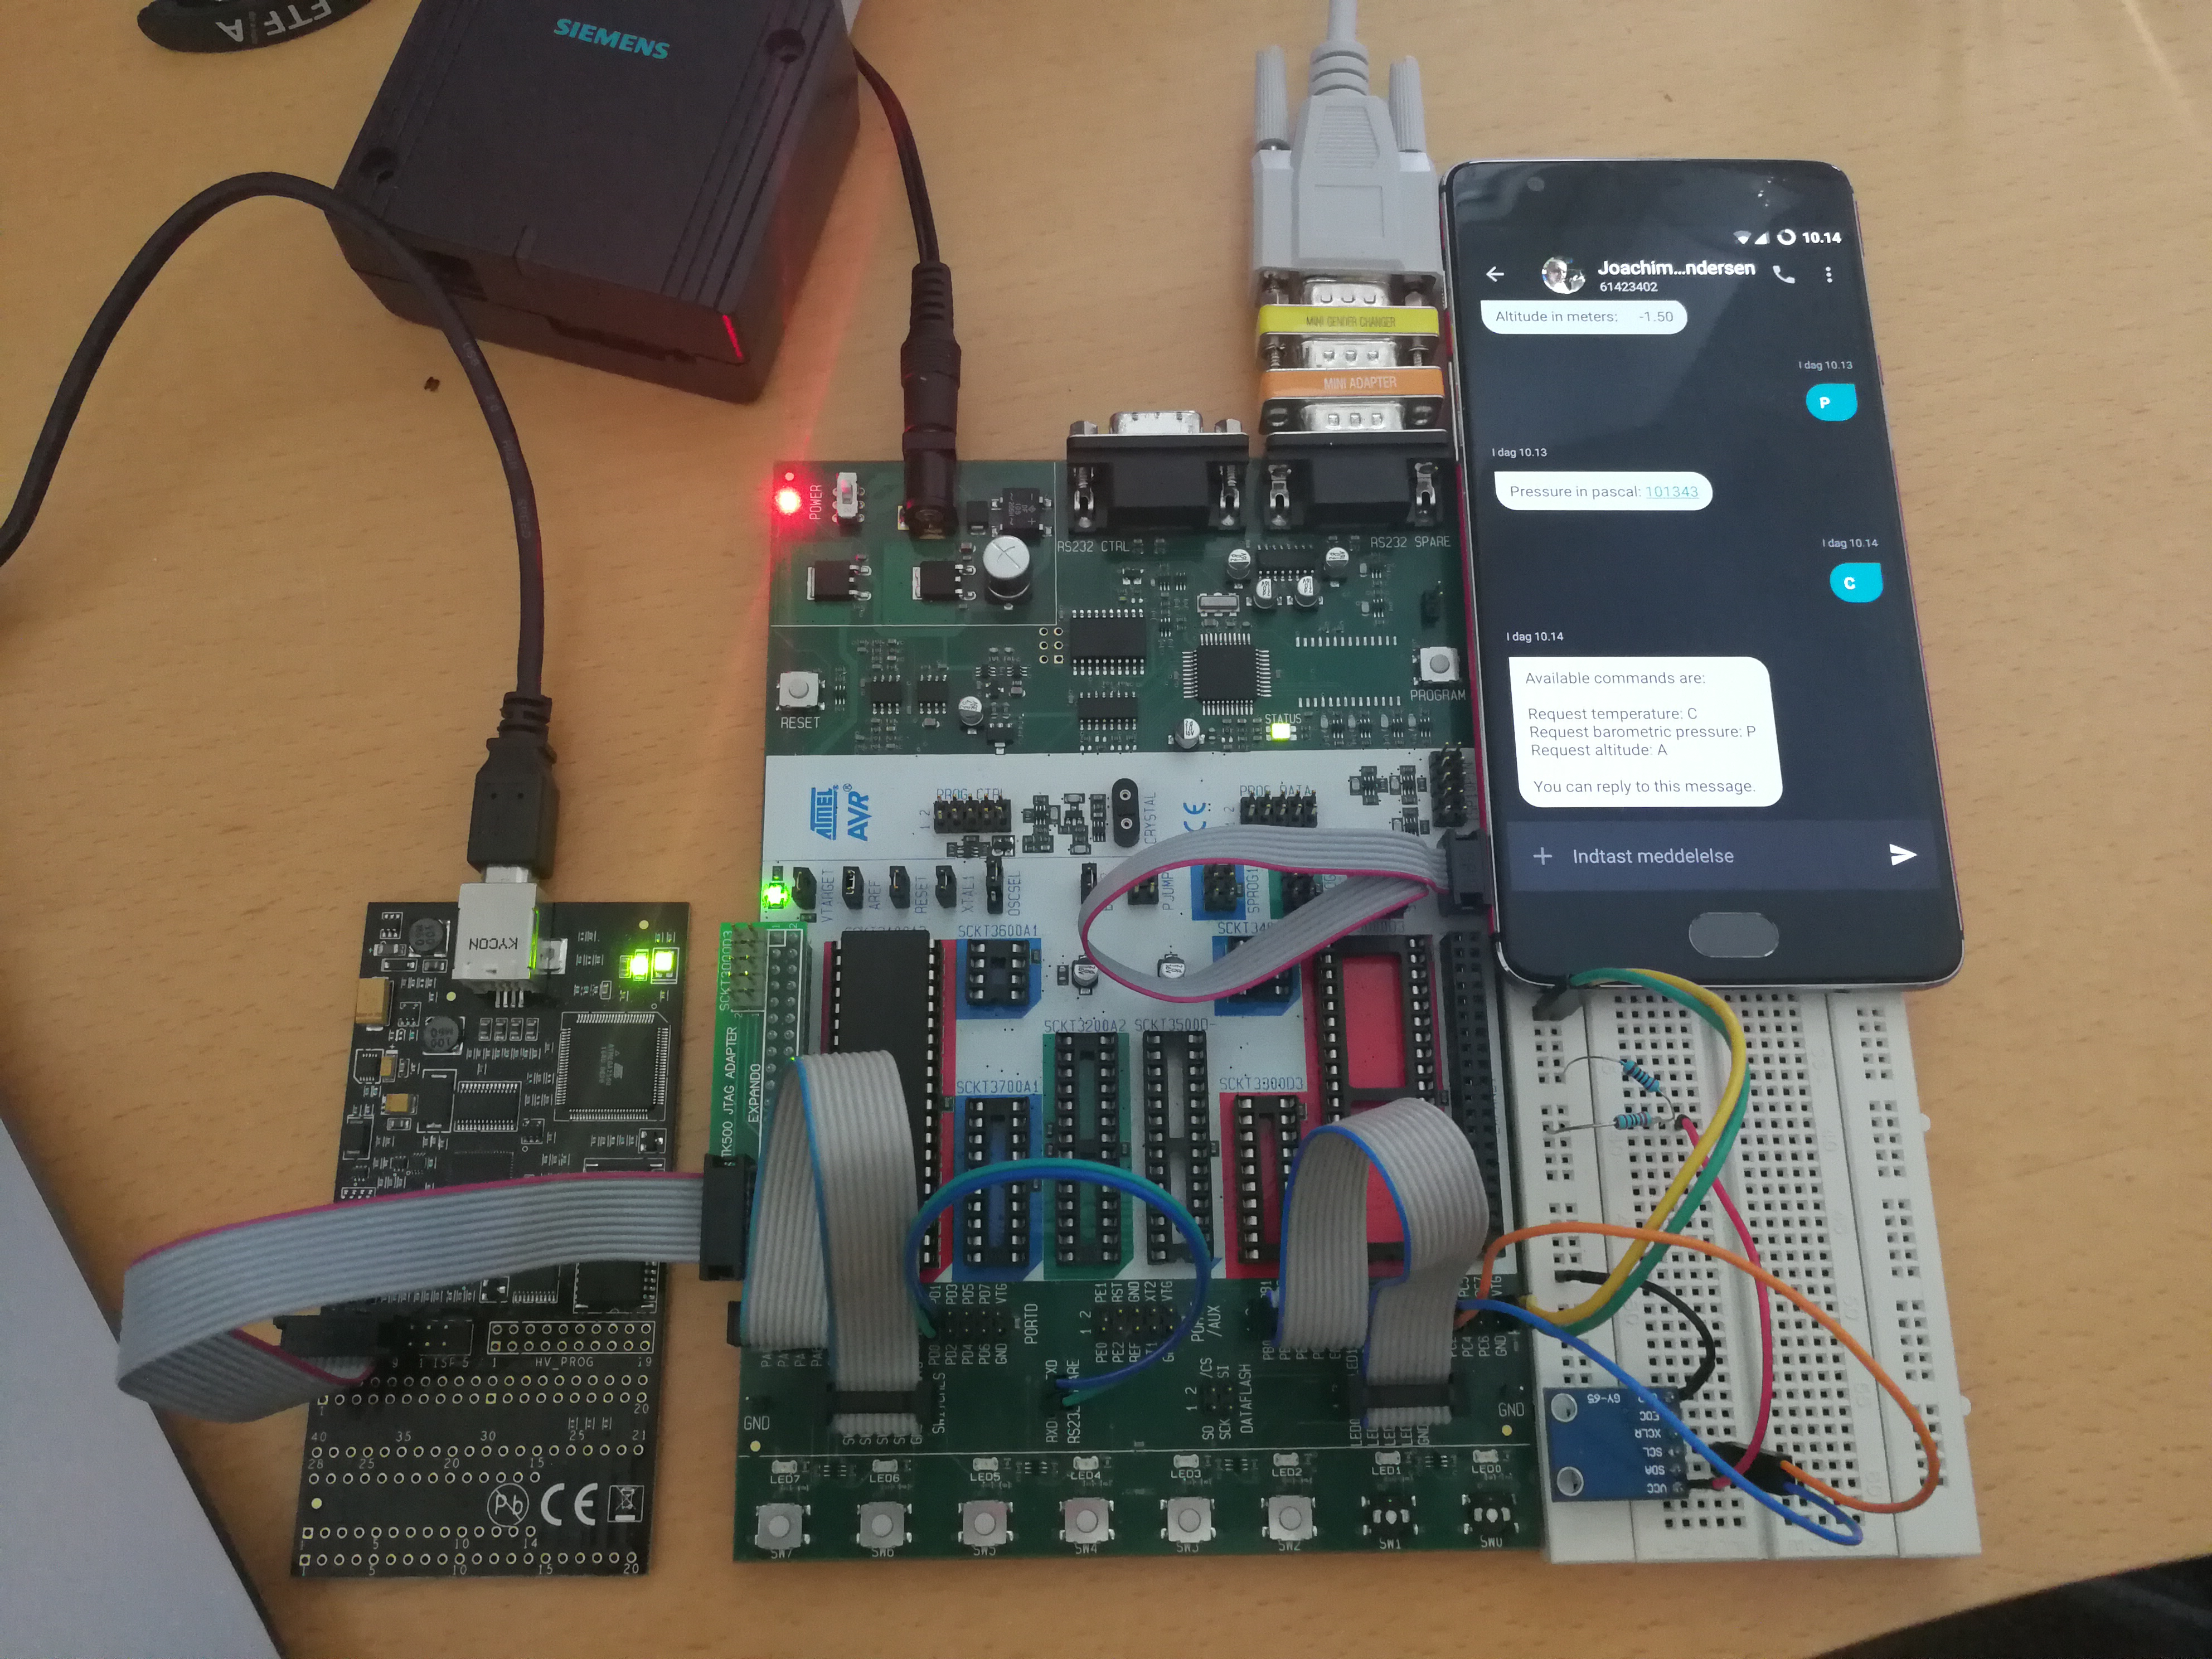
\includegraphics[width=\linewidth]{figs/test_setup}
	\caption{Billede af testopsætning.}
	\label{fig:testsetup}
\end{figure}

\subsection{Demo}
Da demo-guderne næppe tillader at en ''live''-demo går godt, er herunder et link til en YouTube video, som demonstrerer systemet.

\vskip 0.5cm
	\begin{center}
		\url{https://www.youtube.com/watch?v=xx1EggCptEE}
	\end{center}
\vskip 0.5cm

\subsection{Konklusion}

I løbet af dette projekt er det lykkedes at udvikle et system som ved modtagelse af en SMS kan indhente en sensormåling fra ekstern enhed og svare på den oprindelige besked med den ønskede måling. 

Den største udfordring har været at få MC35 GSM modem'ets timings til at stemme med kravene fra fabrikken. Men da disse udfordringer var løst kunne de resterende opgaver relativt hurtigt løses.
Den oprindelige tanke med systemet var at også kunne hente GPS koordinater fra en GPS reciever. Der kunne hentes data fra GPS recieveren gennem UART/USART, men da der som udgangspunkt kun 
er understøttet kommunikation med et enkelt device, blev det besluttet at skrotte ideen med GPS'en og i stedet fokusere på BMP085 sensoren.

Yderligere var det også meningen at der skulle tilsluttes et GPS modul, vist på figur~\ref{fig:gps}, som også kunne anmodes om data. Denne krævede også en UART forbindelse og blev derfor nedprioriteret da det var nødvendigt at lave funktionalitet som muliggør runtime skift mellem UART til BMP og GPS modul. Dog blev der etableret forbindelse til modulet, som vist med terminal print på figur~\ref{fig:gsp_terminal}

Derudover er projektet alt i alt gået godt og den valgte problemstilling er blevet løst efter hensigten. 
